\chapter{Diagrams}

\section{Block view}
The following figure summarizes the main blocks and interactions between sensors, controls, and actuators.

\begin{center}
\resizebox{\textwidth}{!}{%
\begin{tikzpicture}[node distance=2.0cm, auto, thick, scale=0.9, transform shape]
  \tikzstyle{block} = [rectangle, draw, rounded corners, align=center, minimum width=2.4cm, minimum height=1cm]

  \node[block] (sensors) {Sensors\\NTC, DHT22, LDR, Buttons};
  \node[block, right=2.5cm of sensors] (control) {Controls\\Thermostat, Humidifier, Lighting, Turnstile};
  \node[block, right=2.5cm of control] (act) {Actuators\\LED, PWM, Servo};
  \node[block, below=1.6cm of control] (ui) {LCD Display\\Status and diagnostics};

  \draw[->] (sensors) -- (control);
  \draw[->] (control) -- (act);
  \draw[->] (control) -- (ui);
\end{tikzpicture}%
}
\end{center}

\section{Loop logical sequence}
The update cycle is designed so the display always shows the most recently computed state.

\begin{center}
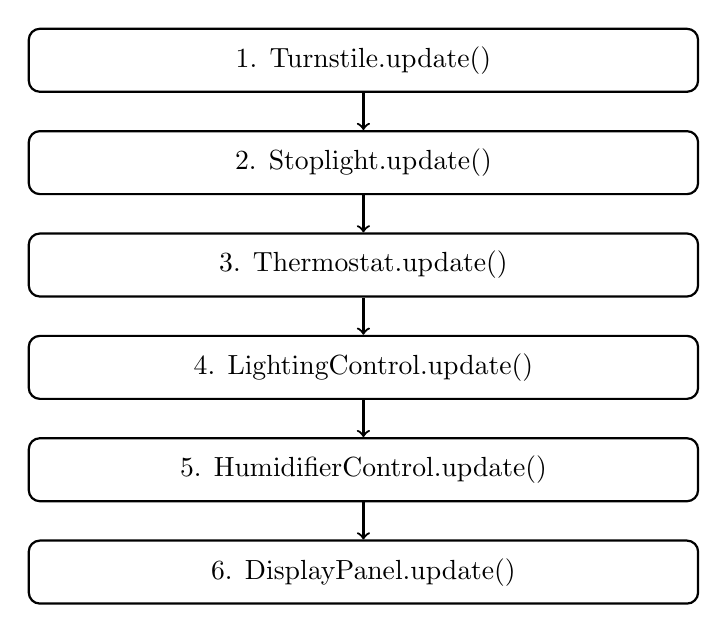
\begin{tikzpicture}[node distance=1.3cm, auto, thick]
  \tikzstyle{stepbox} = [rectangle, draw, rounded corners, align=center, minimum width=8.5cm, minimum height=0.8cm]

  \node[stepbox] (s1) {1. Turnstile.update()};
  \node[stepbox, below of=s1] (s2) {2. Stoplight.update()};
  \node[stepbox, below of=s2] (s3) {3. Thermostat.update()};
  \node[stepbox, below of=s3] (s4) {4. LightingControl.update()};
  \node[stepbox, below of=s4] (s5) {5. HumidifierControl.update()};
  \node[stepbox, below of=s5] (s6) {6. DisplayPanel.update()};

  \draw[->] (s1) -- (s2);
  \draw[->] (s2) -- (s3);
  \draw[->] (s3) -- (s4);
  \draw[->] (s4) -- (s5);
  \draw[->] (s5) -- (s6);
\end{tikzpicture}
\end{center}
